\documentclass{article}
\usepackage[utf8]{inputenc}
\usepackage{../../utils/personalmacros}

\title{Algorithmics Exercise 1}
\author{Konstantin Mark}
\date{October 2022}

\begin{document}

\maketitle

\begin{exercise}[$A*$ Algorithm]
    Perform the $A*$ Algorithm on the following graph in order to find a shortest path from $s$ to $t$. In which order are the nodes expanded, and when are which nodes reached? Show the content of the priority queue at each iteration.

\begin{figure}[H]
    \centering
    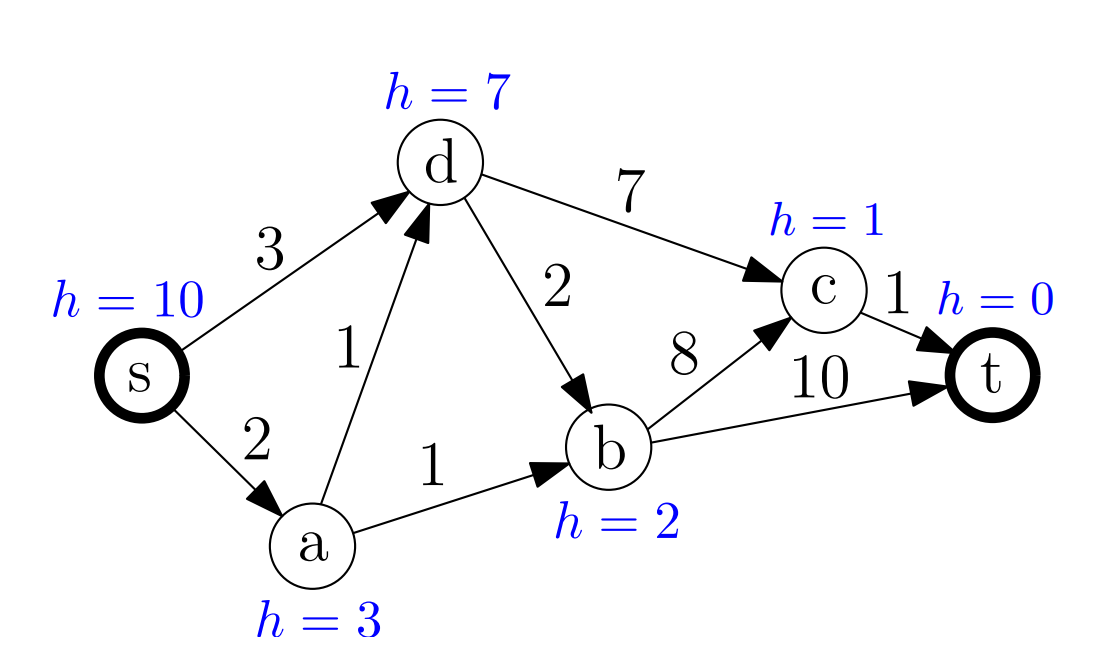
\includegraphics[scale=0.3]{1/exercise/ex1graph.png}
    
    \label{fig:ex1graph.png}
\end{figure}


\end{exercise}
\begin{solving}
    A quick implementation of a graph class with a $A*$-method was done in python. See notebook and code. This leads to the following Output:
    \begin{verbatim}
Start heap:  [(0, 's')]
coming from s to d
the heap is now:  [(10, 'd')]
coming from s to a
the heap is now:  [(5, 'a'), (10, 'd')]
coming from a to b
the heap is now:  [(5, 'b'), (10, 'd')]
coming from b to c
the heap is now:  [(10, 'd'), (12, 'c')]
coming from b to t
the heap is now:  [(10, 'd'), (12, 'c'), (13, 't')]
coming from d to c
the heap is now:  [(11, 'c'), (13, 't'), (12, 'c')]
coming from c to t
the heap is now:  [(11, 't'), (13, 't'), (12, 'c')]
Found path with cost 11
\end{verbatim}
\end{solving}
\newpage

\begin{exercise}[$A*$ Admissible/Monotonic Heuristics]
    Argue whether or not the heuristic function in the above example is admissible and/or monotonic. Consider the $8$-Puzzle discussed in the lecture. Show whether or not the two suggested heuristics $h_1$ and $h_2$ are admissible and/or monotonic
\end{exercise}
\begin{solving}~
\begin{itemize}
    \item Example above:
        \begin{itemize}
            \item Admissibility: The heuristic function is 
            \begin{verbatim}
                h = {'s': 10, 'a': 3, 'b': 2, 'c': 1, 'd': 7, 't': 0 }\end{verbatim}
            and the true minimal cost (very inefficiently calculated by applying the above implementation of $A^*$ to node $t$ with all nodes as starting nodes respectively is \begin{verbatim}
                h_star = {'s': 10, 'd': 10, 'a': 5, 'b': 5, 'c': 11, 't': 11}\end{verbatim}
            and we see that $h\leq h^*$, thus the heuristic is admissible for this graph for the node $t$.\footnote{Question that now came up while working on the problem sheet: Does it happen that the heuristic is defined as a function of two variables, i.e. admissibility then means that $\forall x,t \in V: h(x,t)\leq h^*(x,t)$}
            \item Monotonicity: Since $h(s) = 10 > 5 = 2+3 = w_{s,a} +  h(a)$, this heuristic is not monotonic.
    \end{itemize}
    \item 8-tile, number of tiles in wrong positions:
    \begin{itemize}
        \item Admissibility: Clearly you have to make more moves than the number of tiles that are in a wrong position at any certain point in time as you can only correct one tile per move.
        \item Monotonicity: Let $y$ be reachable from $x$ in one move, i.e. $w_{x,y} = 1$. Now moving the tiles from state $x$ to state $y$ can decrease the number of tiles in a wrong position by a maximum of one, thus $h(x) \leq h(y) + 1  = h(y) + w_{x,y}$
    \end{itemize}
    \item 8-tile, sum of Manhattan distances of each tile to its target location \begin{itemize}
        \item Admissibility: The heuristic gives the number of moves needed if you could move the tiles freely (i.e. moving one tile over another) so clearly, it is smaller than the optimal number of moves needed.
        \item Monotonicity: As before, we can only decrease the distance by one in every move, same argument as in previous example.
    \end{itemize}
\end{itemize}
    
\end{solving}
\newpage

\begin{exercise}[$A*$ Algorithm for an Euclidean Graph]
    Consider an undirected graph whose nodes correspond to points in the Euclidean plane. Instead of directly applying the Euclidean distance in a heuristic $h(x)$, we multiply it by a factor $\alpha>1$, i.e.,
    \begin{equation*}
        h(x) = \alpha \cdot \sqrt{
            (x_1-t_1)^2+(x_2-t_2)^2
        },   
    \end{equation*}
    where $x= (x_1,x_2)\in V$ is an arbitrary node and $t= (t_1,t_2)$ the target node. What might be a motivation for doing this? Is the corresponding $A*$ algorithm still guaranteed to yield a shortest path? Prove or disprove this. How about monotonicity?
\end{exercise}
\newpage

\begin{exercise}[Planar Bipartite Graphs]\label{ex:planBipGraphs}
    Show that $|E|\leq 2|V| - 4$ holds for any simple planar bipartite graph with $|V|\geq 3$ vertices and $|E|$ edges.
\end{exercise}
\begin{solving}
    As we are discussing a planar graph, we can talk about faces. Denote the number of faces as $f$. As the graph is bipartite, any face must be bounded by an even number of edges, thus, the number of edges per face is at least 4. Each edge can only bound at most 2 faces. Thus, $|E|\geq \frac{4f}{2} = 2f$. Now,\begin{itemize}
        \item if $G$ is a connected graph, then Euler's Formula gives $|V|-|E| + f = 2$. Thus, \begin{equation*}
            2+  |E| -|V| = f \leq \frac12 |E|
        \end{equation*}
        or when rearranged, $|E|\leq 2|V|-4$.
        \item In the case that $G$ is disconnected, look at the connected components $(V_1,E_1), \dots, (V_n, E_n)$. Then \begin{equation*}
            |E| = \sum_{i=1}^n |E_n| \leq \sum_{i=1}^n\left( 2|V_i| - 4\right) = 2|V|-4n \leq 2|V|-4.
        \end{equation*}
    \end{itemize}
\end{solving}
\newpage

\begin{exercise}[Non-planarity of Bipartite Graph $K_{3,3}$]
    Prove that the bipartite complete graph $K_{3,3}$ is not planar, i.e., it is not possible to draw the graph in the Euclidean plane without crossing edges.\\
    Do this without using the above property (Exercise \ref{ex:planBipGraphs}), Kuratowski's theorem, and Wagner's theorem.
    \[\begin{tikzcd}
	A && B \\
	C && D \\
	E && F
	\arrow[no head, from=1-1, to=1-3]
	\arrow[no head, from=2-3, to=1-1]
	\arrow[no head, from=1-1, to=3-3]
	\arrow[no head, from=1-3, to=2-1]
	\arrow[no head, from=1-3, to=3-1]
	\arrow[no head, from=2-1, to=2-3]
	\arrow[no head, from=3-1, to=3-3]
	\arrow[no head, from=2-1, to=3-3]
	\arrow[no head, from=2-3, to=3-1]
\end{tikzcd}\]
\end{exercise}
\begin{solving}
    
\end{solving}

\newpage
\begin{exercise}[Miller-Rabin Primality Test]
    The primality test of Miller-Rabin uses a function $Witness(a,n)$, which checks for two positive integer numbers $a$ and $n$ if 
    \begin{equation*}
        a^{n-1} \equiv 1 \mod n
    \end{equation*}
    holds. Perform this algorithm for $a = 11$ and $n = 161$. Write down the values of all variables for each iteration. What can you conclude from the result?
\end{exercise}

\begin{exercise}[Randomized Algorithm for $3$-Coloring of a Graph]
    Given an undirected graph $G= (V,E)$, a $3$-Coloring is an assignment of one of three colors, e.g., red, green, or blue, to each node so that two adjacent nodes do not have the same color. In an optimization variant of this problem, we maximize the number of satisfied edges, i.e. $\max|\{(u,v)\in E| u \text{ and } v \text{have different colors}\}|$. Find a simple randomized algorithm that satisfies at least $\frac23$ of all edges in the expected case, if such a solution exists. Prove this expectation. Moreover, either prove that such a solution always exists for any instance or give an example of an instance where this is not the case. What is the asymptotic run time of the algorithm? Is your algorithm a Monte Carlo or a Las Vegas approach?
\end{exercise}

\begin{exercise}
    Continuing with the above example, how can you turn your algorithm into a $\frac23$-approximation algorithm? Moreover, derive a reasonable bound for the expeted runtime of this extended algorithm.
\end{exercise}

\end{document}